\subsection{Robottyper} \label{Robottyper}
Robotter kan klassificeres på forskellige måder afhængigt af den opgave de udfører, miljøet de gør det i, design og autonominiveau. Af de kategorier der er beskrevet i ISO 8373:2021 \parencite{ISO2021ISOVocabulary} og \cite{IFR2023World2023} er der to relevante kategorier for projektet. Desuden er printere og 3D FDM printere også inkluderet, da de udfører lignende opgaver.

\textbf{Industrirobotter} er automatiserede og programmerbare maskiner, der bruges i industrielle miljøer til opgaver såsom samling, svejsning og malerarbejde \parencite{IFR2023World2023}. Industrielle robotter kommer i alle størrelser, men kræver, til forskel fra de andre kategorier, særlig infrastruktur omkring dem. Det kan fx være indhegninger for robot arme, som vist på figur \ref{fig:irb7710pic}. De skal dermed ikke tage højde for mennesker, og bruges ofte til at udføre opgaver, hvor det er for dyrt eller farligt at ansætte folk \parencite{ABB2023IRBSeries, ISO2021ISOVocabulary}. 

\begin{figure}[H]
    \centering
    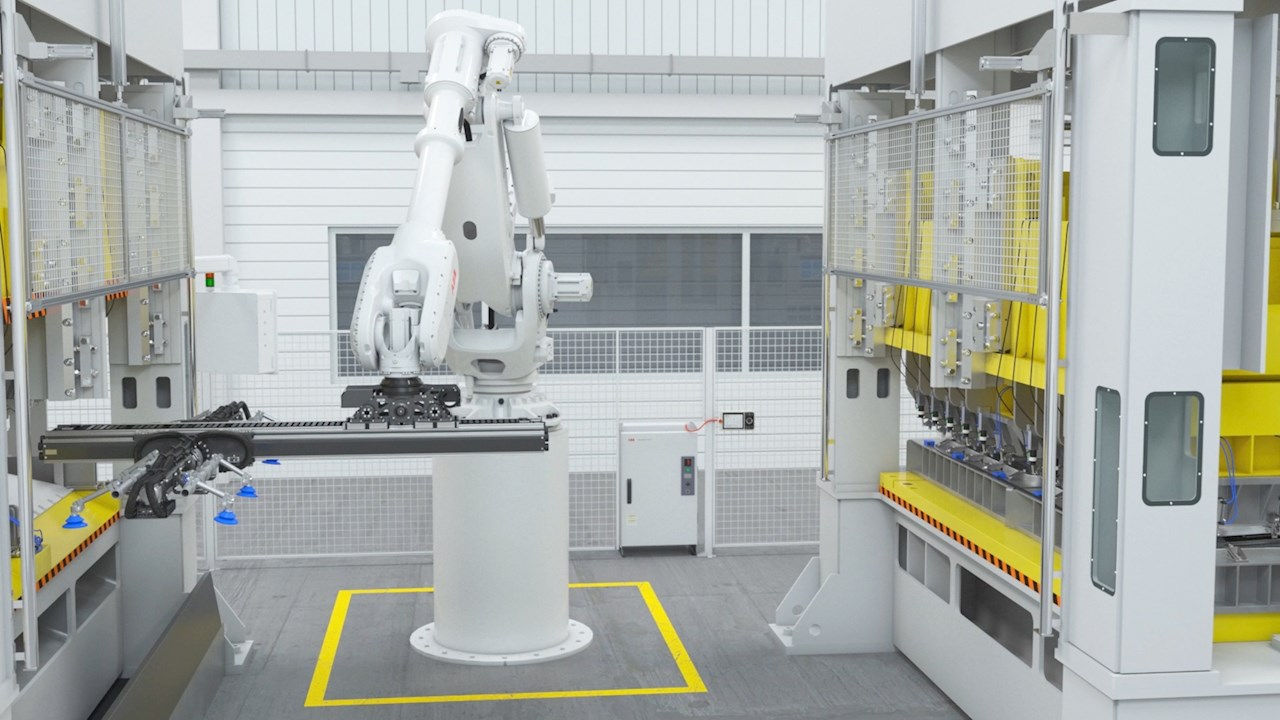
\includegraphics[width=0.6
    \textwidth]{Sections/2 Problemanalyse/Media/irb7710.jpg}
    \caption{IRB-7710 robotarm fra ABB \parencite{ABB2023IRBSeries}}
    \label{fig:irb7710pic}
\end{figure} \plainbreak{-0.5}
\textit{Eksempel:} ABB's IRB-robotter, serien indeholder mange forskellige størrelser af robotter. På figur \ref{fig:irb7710pic} ses model 7710, som er i den store ende og har en løftekapacitet på op til \SI{500}{kg}. På figuren er den sat op til at flytte store plader fra en stor maskine til en anden, robotten er praktisk her, da den kan løfte pladen fra midten af den ene maskine, og placere den i midten af den anden.
    
\textbf{Collaborative Robots (Cobots)} er designet til at arbejde sikkert sammen med mennesker i fælles arbejdsområder. De er ofte udstyret med sensorer og avancerede kontrolsystemer for at sikre at de kan koeksistere sikkert med mennesker \parencite{IFR2023World2023}. Her er sikkerhed altså en meget høj prioritet. Til forskel fra Servicerobotter er denne type ofte mere generaliserede og designet til at kunne arbejde sammen med mennesker, ikke blot i samme miljø.

\begin{figure}[H]
    \centering
    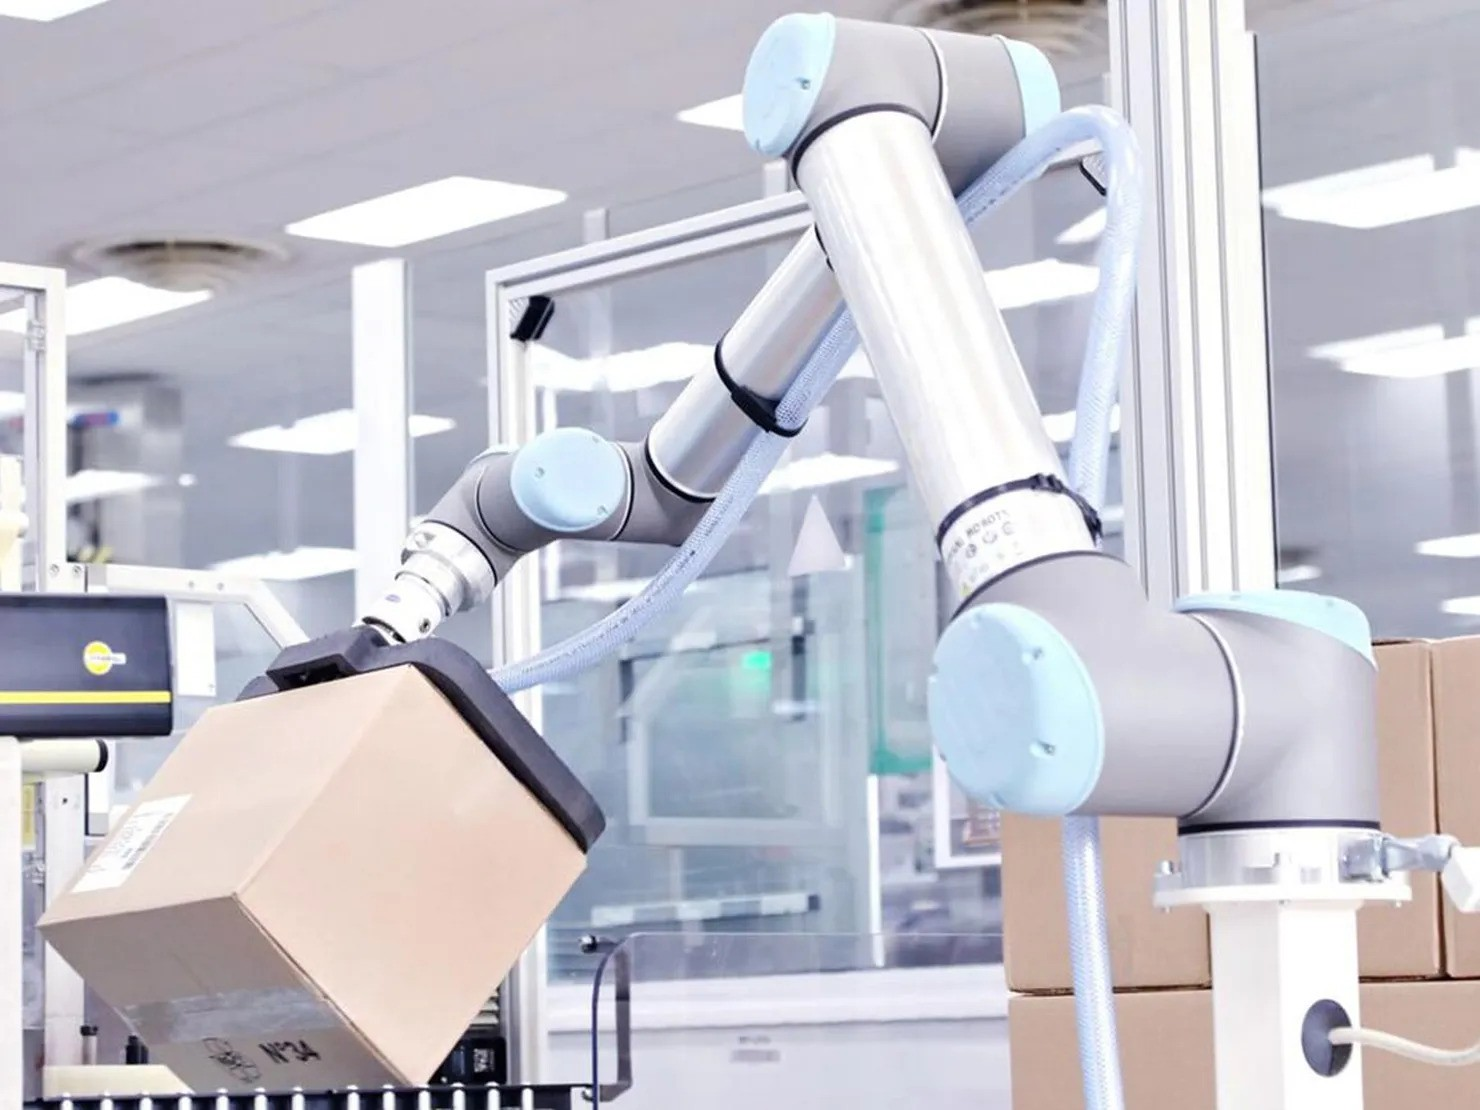
\includegraphics[width=0.5\linewidth]{Sections/2 Problemanalyse/Media/URrobot.jpg}
    \caption{UR5, et letvægt Cobot lavet i Danmark \parencite{2023URSeries}}
    \label{fig:ur5pic}
\end{figure} \plainbreak{-0.5}

\textit{Eksempel:} Universal Robots' UR-serie \parencite{2023URSeries}. Designet til at være flexible, billig og let. Primært tænkt til at samle op, flytte og placere. Fx kan den placere en del foran et mennesker, der kan udføre noget arbejde, hvorefter UR5 kan flytte den væk igen. Cobots bruges altså til at automatisere simple handlinger hvorimod mennesker stadig udføre mere kompliceret arbejde.

\textbf{Printere} er en type maskine, hvor et printhoved bevæger sig hen over en overflade for at afsætte små dråber væske i et præcist mønster. Systemet består typisk af en mekanisk struktur, der styrer printhovedets bevægelser i én retning, mens underlaget enten er stationært eller bevæges i en vinkelret retning. Bevægelsen kontrolleres af motorer, som sikrer en jævn og præcis føring, hvilket gør det muligt at opnå en ensartet fordeling af materialet på overfladen. Afhængigt af konstruktionen kan nogle systemer også bevæge printhovedet i begge retninger og på den måde optimere hastigheden og effektiviteten.\parencite{Delaney2009InkjetProteins} 

\begin{figure}[H]
    \centering
    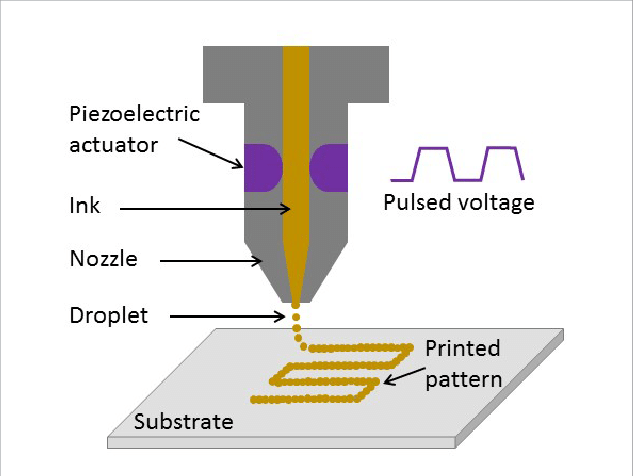
\includegraphics[width=0.5\linewidth]{Sections/2 Problemanalyse/Media/inkjet.png}
    \caption{Illustration af hvordan en Inkjet printer fungere \parencite{Long2025AOptimizations}}
    \label{fig: Inkjet}
\end{figure} \plainbreak{-0.5}

Inkjet-printere anvender dyser, der sprøjter væske ud som små dråber. Størrelsen på disse dråber og afstanden mellem dem bestemmes af både dysens udformning og systemets præstationsniveau, se figur \ref{fig: Inkjet}. Printhovedet kan tilpasses til at håndtere forskellige væsketyper, hvilket gør teknologien fleksibel i forhold til materialevalg. Systemet er primært designet til at arbejde på plane eller næsten plane overflader, da det kræver en ensartet afstand mellem printhovedet og emnet for at sikre korrekt afsætning af materialet.\parencite{Delaney2009InkjetProteins} 

Inkjet-printers bevægelsessystemer er karakteriseret ved høj nøjagtighed og genskabelighed, hvilket gør dem velegnede til opgaver, hvor præcis materialepositionering er nødvendigt. Systemet er ofte simpelt opbygget og kan tilpasse forskellige størrelser afhængigt af anvendelsen. Selvom inkjet-printere ofte anvendes til at printe tekst eller billeder på papir, kan teknologien også tilpasses andre formål, hvor præcis placering af små dråber eller partikler er nødvendigt.

%De andre printerteknologier, laser og termisk, kan allerede nu kasseres da laserprintere vil varme emnet op, og dermed kan ændre emnets egenskaber og termiske printer kun virker da papiret er varmereaktivt. De er derfor ikke relevante.

\textbf{FDM 3D Printere} bruges ofte med et standard kartesisk bevægelsessystem.  Det kartesiske bevægelsessystem for 3D-printeren er kendetegnet ved, at elmotorer kontrollerer bevægelse langs tre akser, x-, y- og z aksen, se figur \ref{fig:3D printer}.

\begin{figure} [H]
    \centering
    \includegraphics[width=0.5\linewidth]{Sections/2 Problemanalyse/Media/3D printer bevægelse.png}
    \caption{3D printer illustration. \parencite{Mueller20203DDraft}. }
    \label{fig:3D printer}
\end{figure}\plainbreak{-0.5}

 De er ofte lavet med bælter eller med en ledeskrue der kan føre printerhovedet i de tre retninger. Dette vil også være en mulig måde at lave en robotbevægelse, til påføring af speckle patterns, på en 2D overflade. \parencite{Billington20243DOverview}